\chapter{Phase de tests}
\label{Chap3}
Nous souhaitons réaliser quelque chose de nouveau et d'assez lourd à mettre en place, nous souhaitons d'abord savoir quels paramètres utiliser pour avoir ce que l'on souhaite. Nous allons réaliser des structures simples à réaliser et à mesurer pour réaliser ces tests. Notre but est de réaliser une jonction entre Cuivre et Aluminium, avec une couche d'oxyde d'Aluminium entre les deux. En effet, les nanofils vont s'oxyder sur durant leur voyage depuis Copenhague, et nous souhaitons savoir comment se débarasser de cette couche d'oxyde.

    %\section{Procédure : Fabrication et mesures}
       % Nous avons commencé par réaliser des tests de manière relativement peu rigoureuse (échantillons peu adaptés, paramètres manquant...), nous ne prendrons pas en compte les résultats de ces tests dans notre analyse, les paramètres étant trop différents.
        %La deuxième série de tests réalisée, beaucoup plus rigoureuse c'est déroulée en prenna
    
    
    \section{Processus de fabrication, influence des paramètres}
    La fabrication d'échantillon se déroule en plusieurs étapes, chacune apportant son lot de paramètres pouvant influer de manière, comme nous le verrons, plus ou moins importante.
    \begin{description}
        \item[$\bullet$ Dépot de résine]{Vitesse de rotation, température de cuisson}
        \item[$\bullet$ EBL]{Dose d'électrons, résolution, energie, forme}
        \item[$\bullet$ Développement]{Durée d'immergement dans MIBK et MethyGlycol}
        \item[$\bullet$ Dépot d'Aluminium]{Angle d'évaporation}
        \item[$\bullet$ Oxydation]{Pression et durée}
        \item[$\bullet$ Plasma Etching]{Pression d'Argon, durée, Voltage, energie des ions}
        \item[$\bullet$ Dépot de Cuivre]{Angle d'évaporation}
        \item[$\bullet$ Lift-off]
        \item[$\bullet$ SEM]
    \end{description}
    
    Les paramètres que nous ferons varier au cours de ces test seront : la forme du pattern (différentes surfaces de jonction : 0.5, 1, 1.5 et 2$\mu m^2$), la dose d'électrons de l'EBL (de 2000 à 3000$\mu c/cm^2$ par pas de 250), et la durée du plasma pour connaître son effet sur la jonction.
        
        \subsection{Temps de développement}
            Le temps de développement, c'est-à-dire le temps pendant lequel la résine est placé dans le MIBK et le Methyglycol, influe globalement sur la qualité des undercuts. Pour le MIBK, il faut un temps suffisant pour que tout le PMMA et le MMA exposé soit dissout, mais pas trop long pour éviter d'agrandir le pattern. De même pour le Methylglycol, il faut un temps suffisant pour avoir des undercuts suffisamment grandes (ie. que le métal ne s'évapore pas sur le MMA.) mais pas trop long pour éviter que le PMMA ne s'affaisse si trop de MMA est dissout. Cette étape a été réalisée avant mon arrivée des valeurs qui fonctionnaient ont été trouvées, je ne m'étendrais donc pas sur cette partie, cependant c'est un paramètre inmportant à prendre en compte, c'est pour cela que je le mentionne. 

        \subsection{Angles d'évaporation}
            A partir du pattern, toutes les surfaces où la résine a été retirée vont être recouvertes de métal. Ainsi, il faut faire attention à l'angle avec lequel on évapore sinon il n'y aura pas de jonction. Le docteur Taupin avait déterminé +14\textdegree  et -14\textdegree comme des angles fonctionnels pour l'évaporation. Cependant, en regardant les images SEM, on se rend compte que la surface de la jonction n'est pas optimale. J'ai donc réalisé quelques calculs pour déterminer un meilleur angle.
            
            \begin{figure}
                \centering
                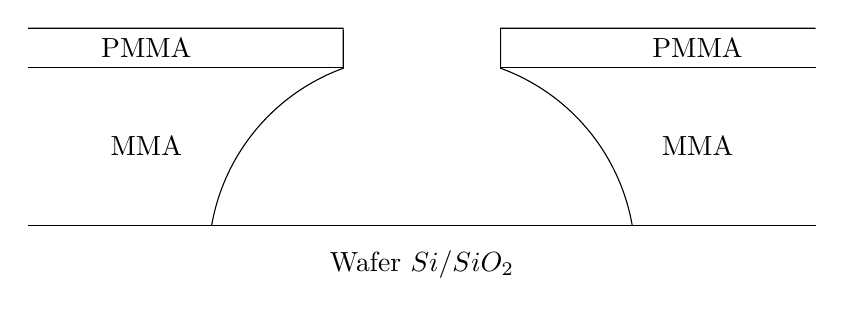
\begin{tikzpicture}
                \draw (0,0)--(10,0);
                \draw (5,-0.5) node{Wafer $Si/SiO_2$};
                \draw (2.33,0) arc(170:110:2.6)--(4,2.5)--(0,2.5);
                \draw (7.67,0) arc(10:70:2.6)--(6,2.5)--(10,2.5);
                \draw (0,2)--(4,2);
                \draw (6,2)--(10,2);
                \draw (1.5,1) node{MMA};
                \draw (8.5,1) node{MMA};
                \draw (1.5,2.25) node{PMMA};
                \draw (8.5,2.25) node{PMMA};
                \end{tikzpicture}
            \end{figure}
        
        \subsection{Durée du plasma}
            Un but annexe que nous nous sommes fixé est de caractériser le plasma, et notamment son utilisation en gravure. D'ordinaire utilisé pour faciliter le lift-off, nous utilisons ici le plasma pour graver l'oxyde d'aluminium. Ainsi, la durée d'exposition au plasma ainsi que l'énergie des ions sont des paramètres importants. 
            
            Détermine la quantité d'Al qui sera gravée. On oxyde fortement l'Al avant de rogner l'oxyde pour revenir en clean contact. En comparant les résistances obtenues à celle sans plasma, on peut déterminer la quantité d'Al$_2$O$_3$ retirée.
            
    \section{Mesures}
        \subsection{Méthode de mesures}
            On réalise des mesures 4 fils sur les jonctions afin de s'affranchir des résistances parasites qui pourraientintervenir. En faisant cela on ne mesure que la résistances de la jonction. Le schéma permettant une telle mesure est le suivant :
            \iffalse
            \begin{figure}
            \centering
            \begin{circuitikz}
            \draw 
        (0,0) node[ground]{} 
            to [V,v=$DC$] (0,3)
            to [R=1<\mega\ohm>] (3,3)
            to [R=10<\kilo\ohm>,*-] (3,0)
            node[ground] {}
        (3,3) to [R=$R_{ech}$,i=$i_{ech}$] (11,3)
            to [ammeter] (11,0) node[ground] {}
        (5,3) to [american resistor, *-] (5,1)
            to [voltmeter, v_>=$V_{ech}$] (9,1)
            to [american resistor, -*] (9,3)            
            ;
            \end{circuitikz}
            \caption{Schéma utilisé pour réaliser des mesures 4 fils}
            \label{Schéma4fils}
            \end{figure}
            \fi
            
            Par la suite, j'ai réalisé des structures à 4 pads de mesures, j'ai donc utilisé une probestation, bien plus adaptée à la réalisation de mesures rapides.
            
        \subsection{Résultats obtenus}
        Les premiers tests réalisés ont été peu rigoureux dans leur manière d'être abordés : échantillons différents, manque de paramètres pris en compte, structures pas adaptées. Ainsi, nous avons mis en place une autre série de tests, plus systématique, et prennant en compte un plus grand nombre de paramètres.
        Nous avons réalisé plusieurs séries de mesures avec des paramètres différents pour tenter de caractériser le plasma de l'évaporateur. La première étape fut de réaliser une jonction $AlCu$ et de mesurer sa résistance. Celle-ci constitue la base de toutes nos mesures. En la retirant, on peut directement associer la résistance résiduelle à l'épaisseur d'oxyde restant, ou bien aux détériorations provoquées par le plasma.
        \begin{figure}
            \centering
            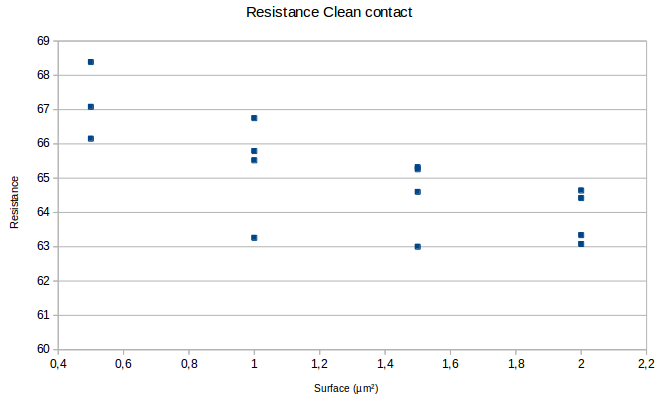
\includegraphics[width=250pt]{RCleancontact.png}
            \caption{Résistance de la jonction Al/Cu en fonction de la surface de la jonction}
            \label{Rclean}
        \end{figure}
        
        Sur la Figure \ref{Rclean}, on remarque que la résistance dépend peu de la surface de la jonction. C'est normal car il s'agit d'un contact propre, c'est à dire un contact entre deux métaux. Ainsi la résistance vaut 
        \[R=\dfrac{\sigma_{Cu} L}{S}+\dfrac{\sigma_{Al} L}{S}\]
        
        Les résistances obtenues pour cet échantillon témoin permettront de connaître la résistance de la partie isolante en la soustrayant, donc l'épaisseur d'oxyde. 
        \section{Interpretation / Conclusions}
        
        \subsection{Influence de la durée du plasma}
        Nous avons pu déterminer comment la durée du plasma influait sur la résistance de la jonction à travers le graphe \ref{RPlasma}. Ceci nous renseigne directement sur l'épaisseur d'oxyde entre les deux métaux et nous permet de savoir quelle durée utiliser pour retirer l'oxyde sur les nanofils.
        \begin{figure}
            \centering
            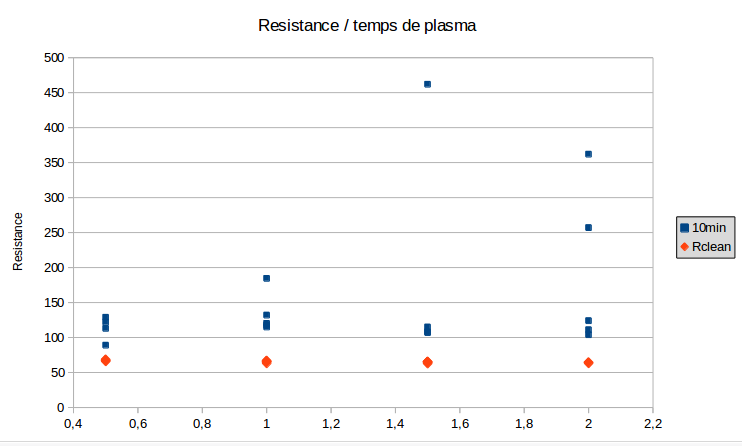
\includegraphics[width=250pt]{RPlasma.png}
            \caption{Résistance mesurée en fonction de la surface de la jonction pour différentes durées de plasma}
            \label{RPlasma}
        \end{figure}
        
        \subsection{Influence de la position de l'échantillon}
        
        Le but secondaire de ces tests était de caractériser le plasma du LISA, l'appareil est relativement récent et on en connait pas tout ces paramètres, cette partie a donc davantage un but communautaire. Le graphe \ref{RPosition} montre la résistance en fonction de la position de l'échantillon sur le porte-échantillon. On remarque que l'ensemble est relativement homogène, le plasma semble donc actif sur la totalité de la zone étudiée.
        \begin{figure}
            \centering
            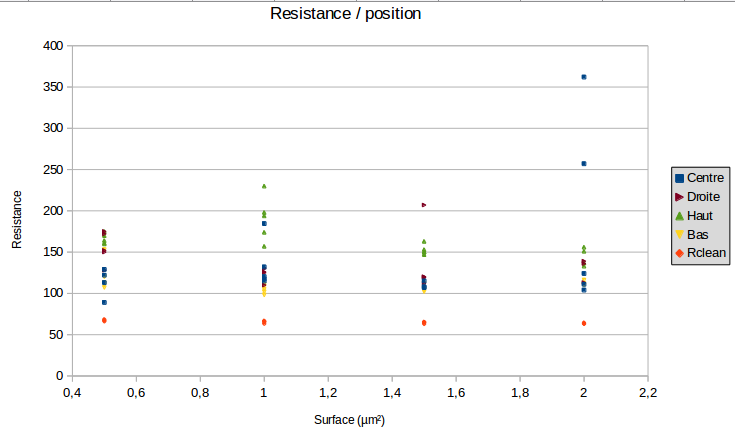
\includegraphics[width=250pt]{RPosition.png}
            \caption{Résistance mesurée en fonction de la surface de la jonction pour différentes positions sur le porte-échantillons}
            \label{RPosition}
        \end{figure}
        
        
        
